%==============================================================================
% Homework X
%==============================================================================


%==============================================================================
% Formatting parameters.
%==============================================================================

\documentclass[11pt]{article} % 10pt article, want AMS fonts.

\usepackage{fullpage}
%\usepackage[top=0.3in, bottom=0.8in, left=0.5in, right=0.5in]{geometry}



%\usepackage{newalg}
\usepackage{amsmath,amsthm, amssymb}
\usepackage{latexsym}
\usepackage{graphicx}
\usepackage{ifthen}
\usepackage{subcaption}
\usepackage{multicol}
\usepackage{algpseudocode, algorithm}
\usepackage[numbers]{natbib}

\newtheorem{lemma}{Lemma}
\newtheorem{theorem}{Theorem}

%==============================================================================
% Macros.
%==============================================================================
%Macros

%Basics
\newcommand{\new}[1]{{\em #1\/}}		% New term (set in italics).

%Probability
\newcommand{\prob}[2][]{\text{\bf P}\ifthenelse{\not\equal{}{#1}}{_{#1}}{}\!\left(#2\right)}
\newcommand{\expect}[2][]{\text{\bf E}\ifthenelse{\not\equal{}{#1}}{_{#1}}{}\!\left[#2\right]}
\newcommand{\var}[2][]{\text{\bf Var}\ifthenelse{\not\equal{}{#1}}{_{#1}}{}\!\left[#2\right]}

%Sets
\newcommand{\set}[1]{\{#1\}}			% Set (as in \set{1,2,3})
\newcommand{\given}{\, : \,}
\newcommand{\setof}[2]{\{{#1} \given {#2}\}}	% Set (as in \setof{x}{x > 0})
\newcommand{\compl}[1]{\overline{#1}}		% Complement of ...            
\newcommand{\zeros}{{\mathbf 0}}
\newcommand{\ones}{{\mathbf 1}}
\newcommand{\union}{{\bigcup}}
\newcommand{\inters}{{\bigcap}}

%Other Math
\newcommand{\floor}[1]{{\lfloor {#1} \rfloor}}
\newcommand{\bigfloor}[1]{{\left\lfloor {#1} \right\rfloor}}
\DeclareMathOperator{\argmax}{argmax}
\DeclareMathOperator{\argmin}{argmin}

%Numbers
\newcommand{\C}{\mathbb{C}}	                % Complex numbers.
\newcommand{\N}{\mathbb{N}}                     % Positive integers.
\newcommand{\Q}{\mathbb{Q}}                     % Rationals.
\newcommand{\R}{\mathbb{R}}                     % Reals.
\newcommand{\Z}{\mathbb{Z}}                     % Integers.
\newcommand{\M}{\mathcal{M}}                     % Matroids.
\newcommand{\I}{\mathcal{I}}                     % Independent Sets.

\newcommand{\bt}{\boldsymbol{\theta}}
\newcommand{\bx}{\mathbf{x}}
\newcommand{\bv}{\mathbf{v}}
\newcommand{\bq}{\mathbf{q}}
\newcommand{\by}{\mathbf{y}}
\newcommand{\bb}{\mathbf{b}}
\newcommand{\bu}{\mathbf{u}}
\newcommand{\bd}{\mathbf{d}}
\newcommand{\ba}{\mathbf{a}}
\newcommand{\bc}{\mathbf{c}}
\newcommand{\bl}{\mathbf{l}}
\newcommand{\bp}{\mathbf{p}}
\newcommand{\bw}{\mathbf{w}}
\newcommand{\bz}{\mathbf{z}}
%Headings
\newcommand{\parta}{\textbf{(a)}}
\newcommand{\partb}{\textbf{(b)}}
\newcommand{\partc}{\textbf{(c)}}
\newcommand{\partd}{\textbf{(d)}}
\newcommand{\parte}{\textbf{(e)}}


%==============================================================================
% Title.
%==============================================================================

\title{Distributed Summarization of Dynamic Data}
\author{Emma Alexander and Eric Balkanski}


\begin{document}



\maketitle


\section{Introduction}

In many large datasets, it is useful to have a summary of its content. One way to build this summary is to select a set of representative samples. For example, given a large collection of images, it might be useful to have a small collection of images that represent the entire dataset. This representative set can be used to communicate an at-a-glance version of the dataset. The problem of finding a good representative set can be formulated as a clustering problem such that the greedy algorithm finds a near-optimal representative subset of the input data. However, clustering algorithms run in quadratic time, which makes the computation aspect of this problem unfeasible for large datasets. \citet{mirzasoleiman2013distributed} show that near-optimal representatives of datasets can be found efficiently with a distributed greedy algorithm both experimentally and theoretically.

Many large real-world datasets are dynamic (Twitter feeds, criminal records, image collections,...) where elements are constantly being inserted and deleted. How should algorithms for data summarization react to such a dynamic setting? In this paper, we explore approaches for this setting with insertions and deletions and their tradeoffs. A (very) naive approach is to run the entire distributed data summarization algorithm for every insertion and deletion. Of course, the communication and computation costs associated with this approach are not desirable, even though it always guarantees a good summarization. Our main interest is in the tradeoff between communication complexity and quality of a summarization. 

\begin{center}
\textit{Can the communication complexity incurred by entirely recomputing a summary at every insertion and deletion be drastically diminished while still maintaining a good summary?}
\end{center}

	
	
	\subsection{Our approach}
	
	In this work, we consider the distributed algorithm for data summarization from \citet{mirzasoleiman2013distributed} and extend it to account for settings with insertions and deletions. Their exact algorithm will be described precisely in Section \ref{s:prelim} and we start by only describing its high level ideas that will be important to discuss our approach. This algorithm first randomly partition the dataset consisting of elements in between multiple local machines. Each local machine computes a set of representatives for the elements it received and sends this set to a central machine. The central machine then aggregates all the local representatives and compute a central solution that is a subset of all these local representatives. This central solution is then the summary of the entire dataset.
	
	Rerunning the entire algorithm at every insertion or deletion would cause every local machine to have to recompute its local solution, send it to the central machine, and the central machine to have to recompute the central solution. The main idea behind our approach is the following simple observation: a local solution does not necessarily need to send its updated local representatives to the central machine at every update.
	
	More precisely, our extension for insertions and deletions use a threshold approach. A local machine only sends to the central machines its updated local representatives when the difference between these representatives and the last set of representatives sent to the central machine exceeds a certain threshold. This approach is quite general, the measure of "difference" and the value of the threshold can be adapted as desired.
	
	To test our approach, we use the dataset of criminal records for the city of Chicago from 2001 to present. Each crime record consists of multiple features and the goal is to find most representative crimes from this dataset. Insertions and deletions are natural since new crimes happen every minute and some records might be erroneous or outdated. Applying the distributed data summarization algorithm to this dataset without updates is of interest in itself since, to the best of our knowledge, this algorithm has never been used for criminal records, but mostly for summarization of collections of images. Our first experiments therefore focus on finding good summaries without updates. The results we obtain make semantic sense (drug related arrests happen on streets and sidewalks, certain neighborhoods have much more crimes than others...) and we believe that they offer a simple and concise representation of the most common crimes in Chicago. Our other experiments focus on understanding the tradeoff between quality of summary and communication complexity. In these experiments, we demonstrate that very good summaries can be maintained with very little communication compared to the communication that would have occurred if a summary would have been recomputed at each insertion and deletion.
	
	\subsection{Previous work}
	
	The distributed algorithm for data summarization that we extend for insertions and deletions is from \citet{mirzasoleiman2013distributed} and is for the general problem of distributed submodular maximization. In subsequent work, instead of picking at most $k$ elements to maximize a submodular function, the question of minimizing the number of elements picked to achieve at least a certain value of a submodular function was studied in a distributed setting \cite{mirzasoleiman2015distributed}. 
	
	An alternate approaches for distributed submodular maximization and distributed clustering uses core-sets (\citet{mirrokni2015randomized, indyk2014composable, balcan2013distributed,bateni2014distributed}). A core-set is a subset of points such that a solution for this core-set is guaranteed to be approximately a good solution for the original set of points.  
	
	A completely different approach to data summarization for very large datasets is via streaming (\citet{badanidiyuru2014streaming,kumar2015fast}). In the streaming model,  elements arrive one by one in a stream and the algorithm maintains a small subset of the elements as the solution while never having access to the entire data set at the same time. A main difference between streaming algorithms and our approach to insertions is that the goal of streaming algorithms is to obtain a good solution when the stream ends and that it is assume to have finite length. We are interested in having a good solution at anytime and we allow for an unbounded number of insertions.
	
	\subsection{Paper organization}
	
	Preliminaries are in Section~\ref{s:prelim}. We then describe and discuss our approach in Section~\ref{s:approach}. We demonstrate the effectiveness of our approach with experiments on a real world criminal dataset in Section~\ref{s:experiments}. Finally, we briefly discuss how to achieve fault tolerance in Section~\ref{s:failures}.
\section{Preliminaries}
\label{s:prelim}
\subsection{Setup} There is a ground set $N = \{e_1, \ldots, e_n\}$ of elements. The goal is to pick a small set $S \subseteq N$ of size at most some integer $k$ that is a good summary of $N$. To measure the quality of a summary, we consider a clustering function measuring the loss $l(S)$ associated with a metric distance $d(e_i, e_j)$. The distance $d(e_i, e_j)$ between two elements $e_i$ and $e_j$ measures how similar these two elements are, this distance function is general and defined differently for different applications. An example of a distance function in the case where elements consists of multiple feature is the hamming distance between these two elements, i.e., how many features they differ on. Once we have a distance function, the clustering function loss $l(S)$ is then the sum over all elements in  $N$ of their distance to their best representative, i.e.,
%
$$l(S) = \sum_{e_i \in N} \min_{e_j \in S} d(e_i, e_j).$$
%



\subsection{Submodularity}
The objective function $f(S)$ is then defined to be 
%
$$f(S) := l(e_0) - l(S \cup e_0)$$
%
 for some auxiliary element $e_0$. The motivation for this definition is that $f(S)$ is monotone submodular. Submodularity is the desirable property of diminishing marginal return. Submodularity is desirable because it allows for theoretical guarantees. More precisely, the simple greedy algorithm is a $e/(e-1)$ approximation algorithm for maximizing a submodular function $f(S)$ under a cardinality constraint, i.e., 
 $$
 \max_{\substack{|S| \leq k \\ S \subseteq N}}f(S).
 $$
 Our goal is therefore a distributed algorithm for this optimization problem with the above definition of $f(S)$ and where insertions and deletions on the ground set $N$ of elements occur.

\subsection{Approximation ratio} The performance of an algorithm, i.e., the quality of the summary it computes, is measured by the approximation ratio $\alpha$ obtained by this algorithm, which is the ratio of the value of the optimal solution to the value of the solution it computes. More precisely, let $S$ be the set returned by an algorithm, this solution is an $\alpha$-approximation if 
%
$$\alpha \cdot  f(S) \geq f(S^\star)$$
%
where $S^{\star}$ is the optimal solution to the problem. An algorithm is then an $\alpha$-approximation algorithm if it is guarantees to always return a solution that is an $\alpha$-approximation, for all inputs.

\subsection{Non-dynamic algorithm}

We now formally describe the algorithm from \citet{mirzasoleiman2013distributed} for distributed submodular maximization that does not deal with insertions and deletions. The ground set $N$ is partitioned into $m$ parts $V_1, \ldots, V_m$. There are $m$ \emph{local machines} each containing a part $V_i$. Each local machine runs the greedy algorithm on its part $V_i$ and obtains a \emph{local solution} $S_i \subseteq V_i$ of size $k$. Each local machine then sends its local solution to the \emph{central machine}. The central machine then aggregates all local solutions and computes a \emph{central solution} by running the greedy algorithm to pick a subset $S \subseteq \cup_i S_i$ that best represents a subset $V$ of the ground set $N$ that the central machine has access to.

By exploiting the submodularity of the problem, the above approach is a $e / ((e-1) \cdot \max(m,k))$ approximation algorithm for the general case of submodular function. This approximation ratio is improved for datasets with certain geometric structures and/or very large datasets. In addition to theoretical guarantees, the effectiveness of this distributed algorithm is also demonstrated with experiments on large collections of images.
\section{Our Approach}
\label{s:approach}
\section{Experiments}
\label{s:experiments}

Semantically, we found that our system's results were reasonable. The crimes were well-distributed, repeated crimes were generally quite different (a common feature was that battery would be repeated, with domestic events in the home showing up separately from nondomestic outdoor battery leading to arrest), but also showed that some times of day and districts were more or less likely to contain crime (e.g. few afternoon crimes, multiple representatives from ``bad neighborhoods"). A sample set of 10 representatives is shown, in no particular order, in Figure \ref{tab:1}.

\begin{figure}
\begin{tabular}{cccccc}
Time of Day & Crime & Location & Arrest & Domestic & District \\
\hline
EVENING & BATTERY & RESIDENCE & false & false & 006 \\
NIGHT & NARCOTICS & STREET & true & false & 011\\
NIGHT & THEFT & STREET & false & false & 004\\
EARLY MORNING & CRIMINAL DAMAGE & APARTMENT & false & false & 007\\
EVENING & NARCOTICS & SIDEWALK & true & false & 011\\
NIGHT & BATTERY & APARTMENT & false & true & 006\\
AFTERNOON & THEFT & STREET & false & false & 025\\
MORNING & BURGLARY & RESIDENCE & false & false & 009\\
NIGHT & BATTERY & SIDEWALK & false & false & 012\\
EVENING & BATTERY & RESIDENCE & false & true & 004\\
\hline
\end{tabular}
\caption{A summary of crimes in Chicago of size 10.}
\label{tab:1}
\end{figure}


Quantitatively, we tested the performance of our algorithm for several thresholds $t$ (see Section~\ref{s:approach} for definition), finding 10 representatives initialized on 300 entries from the Chicago crime dataset with 2 local processes, as 200 insertions were performed. We only used 2 local processes to maximize the impact of a small number of insertions or deletions. On each insertion, the central solution corresponding to each threshold was scored, as was the oracle solution (defined below). The raw scores (defined below) are shown in Figure \ref{fig:scores} for each insertion and threshold.
\begin{itemize}
\item \textbf{Raw score.} The raw score, also called $f$ score, of a set $S$ obtained is simply the value $f(S)$ where $f(\cdot)$ is defined in Section~\ref{s:prelim} and that we aim to maximize.

\item \textbf{Oracle score.} The raw score obtained by running the greedy algorithm on the entire dataset.

\item \textbf{Approximation ratio.} Note that it is computationally unfeasible to find the optimal solution maximizing $f(\cdot)$, we therefore use the oracle score as a proxy for the optimal solution when measuring approximation ratios, defined in Section~\ref{s:prelim}. Recall that we wish to minimize the approximation ratio.
\end{itemize}

In black, the oracle's solution improves steadily, while in black stars a naive never-update algorithm is shown to perform better than one might expect, given the near-doubling of the dataset. The colored lines in between show that by using a threshold, performance can be increased even to level of the global greedy solution with far less frequent communication. More revealing is the approximation ratio between the oracle and central scores, shown in Figure \ref{fig:ratio}.

\begin{figure}
    \centering
    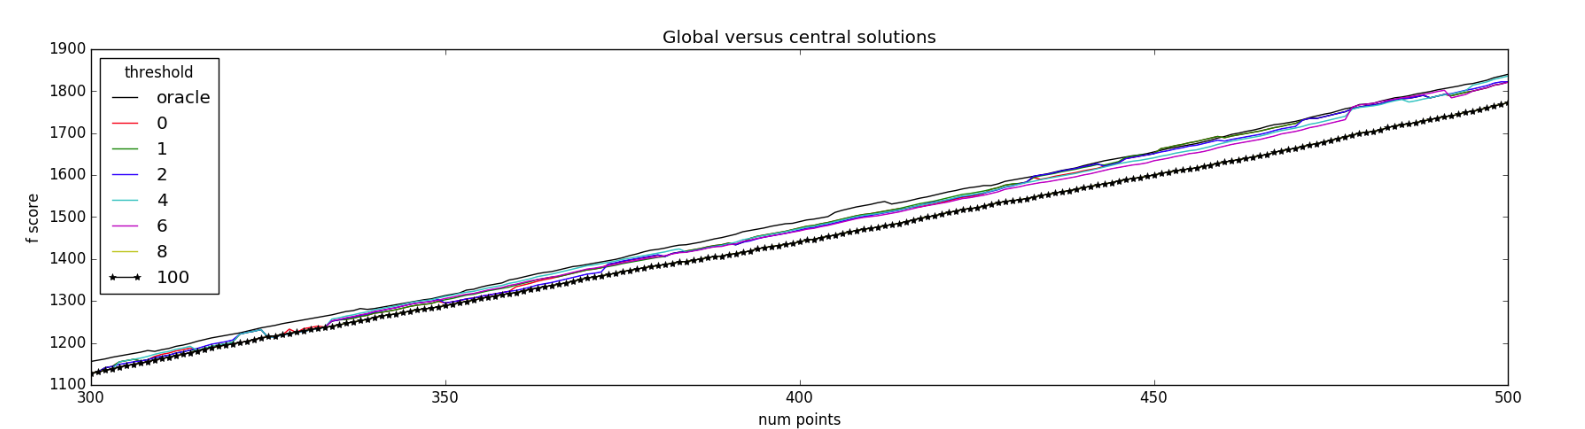
\includegraphics[width=\linewidth]{scores}
    \caption{Raw scores for solutions found under varying thresholds $t$ (colors), effectively infinite solution (black with stars), and with access to all data (black line).}
    \label{fig:scores}
\end{figure}

\begin{figure}
    \centering
    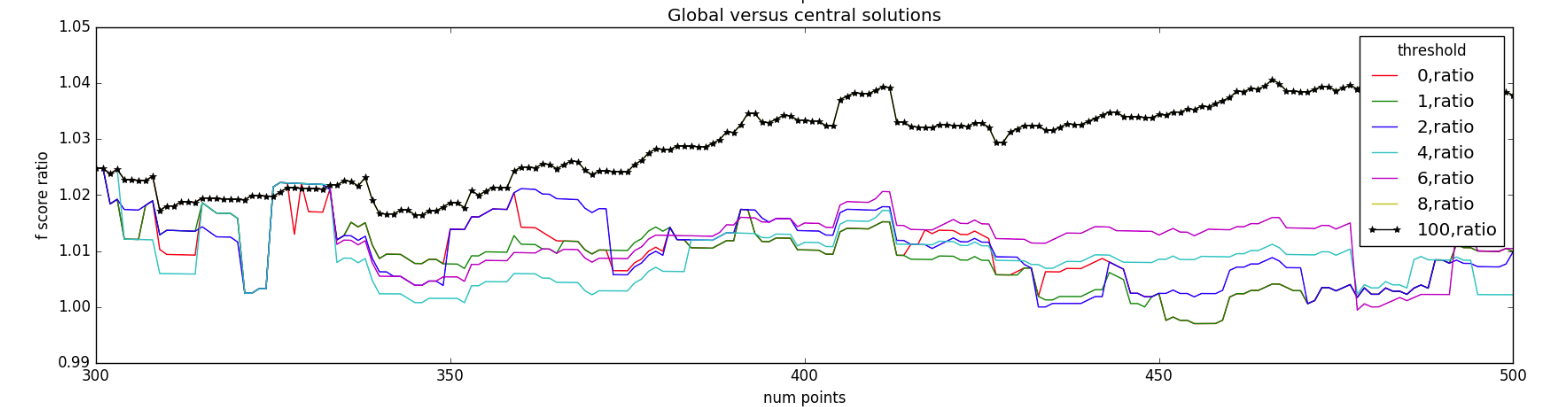
\includegraphics[width=\linewidth]{ratio}
    \caption{Approximation ratios obtained from figure \ref{fig:scores}.}
    \label{fig:ratio}
\end{figure}

This measurement, for which 1 is optimal and lower numbers indicate better performance, shows that thresholds improve performance over the naive baseline, though their ordering is fairly variable. We even see the thresholded performance underperforming the naive solution near 330 entries. This plot tells us that a threshold can be expected to usually but not strictly improve performance, and that in the case of this dataset the threshold can exceed half of the representatives (6 changes out of 10) without a serious loss in performance. The threshold of 8 cannot be seen in this plot because it is identical to the naive never-update performance, indicating a major change in behavior between these settings. Finding this tradeoff point for other datasets will determine the lowest communication cost for sensitivity to data changes.

For details on the generation of these plots and the underlying data, see the README file on github.




\end{document}

